% Image Super-Resolution — A0 LANDSCAPE presentation poster
% Same design and same type sizes as the original portrait poster; only the page
% shape changed, and the qualitative crops now run full width so they render large.
% Compile with pdflatex (needs: beamerposter, tcolorbox, booktabs, tikz)
\documentclass[final]{beamer}
\usepackage[size=a0,orientation=landscape,scale=1.35]{beamerposter}
\usepackage{graphicx}
\usepackage{booktabs}
\usepackage{tikz}
\usetikzlibrary{arrows.meta,positioning}
\usepackage[most]{tcolorbox}
\usepackage{helvet}
\renewcommand{\familydefault}{\sfdefault}

% ---- colors (VUB identity) ----
\definecolor{vubblue}{RGB}{20,61,120}
\definecolor{vubblue2}{RGB}{31,79,150}
\definecolor{vuborange}{RGB}{238,108,30}
\definecolor{cardborder}{RGB}{221,226,234}
\definecolor{inkmuted}{RGB}{91,106,128}
\definecolor{pagebg}{RGB}{245,246,248}

\setbeamertemplate{navigation symbols}{}
\setbeamercolor{background canvas}{bg=pagebg}

% ---- card style ----
\newtcolorbox{card}[1][]{enhanced, colback=white, colframe=cardborder,
  boxrule=1.5pt, arc=0pt, left=14pt, right=14pt, top=12pt, bottom=12pt, #1}

\begin{document}
\begin{frame}[t]

% ================= HEADER =================
\begin{tcolorbox}[colback=vubblue, colframe=vubblue, arc=0pt, boxrule=0pt,
                  left=28pt, right=28pt, top=22pt, bottom=18pt]
  \begin{minipage}[b]{0.76\linewidth}
    {\color{vubblue!30!white}\Large\bfseries DEEP LEARNING PROJECT\; \textperiodcentered\; DIV2K\; \textperiodcentered\; EDSR}\\[0.4ex]
    {\color{white}\veryHuge\bfseries IMAGE SUPER-RESOLUTION {\color{vuborange!80!white}$\times$4}}\\[0.6ex]
    {\color{vubblue!20!white}\large From a low-resolution image to a sharp $\times$4 reconstruction, learned from data.}
  \end{minipage}\hfill
  \begin{minipage}[b]{0.22\linewidth}
    \raggedleft
    {\color{white}\LARGE\bfseries VUB}\\[0.5ex]
    {\color{vubblue!20!white}\large Jawad Shaissah\\ Hamed Nikoo\\ Fahimeh Safari Moghadam}
  \end{minipage}
\end{tcolorbox}
\vspace{-1.2ex}
{\color{vuborange}\rule{\linewidth}{6pt}}

\vspace{0.8em}

% ================= TOP ROW: stats | pipeline =================
\begin{columns}[t]

\begin{column}{0.475\linewidth}
  \begin{columns}[t]
    \begin{column}{0.485\linewidth}
      \begin{card}
        {\color{vubblue}\VERYHuge\bfseries +2.32 dB}\\[0.3ex]
        {\color{inkmuted}\large\bfseries Y-PSNR over bicubic\; \textperiodcentered\; 30.41 dB}
      \end{card}
    \end{column}
    \begin{column}{0.485\linewidth}
      \begin{card}
        {\color{vubblue}\VERYHuge\bfseries $-$32\%}\\[0.3ex]
        {\color{inkmuted}\large\bfseries LPIPS $\downarrow$\; \textperiodcentered\; 0.2804 vs 0.4139}
      \end{card}
    \end{column}
  \end{columns}

  \vspace{0.8em}

  \begin{card}
    {\color{vubblue}\Large\bfseries DIV2K $\times$4\; \textperiodcentered\; 100 held-out test images}\\[0.8ex]
    \renewcommand{\arraystretch}{1.25}
    \begin{tabular*}{\linewidth}{@{\extracolsep{\fill}}l r r r@{}}
      \toprule
       & \textbf{Y-PSNR} & \textbf{Y-SSIM} & \textbf{LPIPS} $\downarrow$\\
      \midrule
      Bicubic                   & 28.09 & 0.7744 & 0.4139\\
      SRCNN                     & 27.15 & 0.7780 & --\\
      VDSR                      & 28.00 & 0.7960 & --\\
      \midrule
      EDSR                      & {\color{vubblue}\textbf{30.41}} & \textbf{0.8371} & {\color{vubblue}\textbf{0.2804}}\\
      + 8$\times$ self-ensemble & {\color{vuborange}\textbf{30.48}} & \textbf{0.8384} & 0.2828\\
      \bottomrule
    \end{tabular*}
  \end{card}
\end{column}

\begin{column}{0.505\linewidth}
  % pipeline
  \begin{tcolorbox}[colback=vubblue, colframe=vubblue, arc=0pt, boxrule=0pt,
                    left=14pt, right=14pt, top=12pt, bottom=12pt]
    {\color{white}\Large\bfseries EDSR PIPELINE}\\[1.0ex]
    \resizebox{\linewidth}{!}{%
    \begin{tikzpicture}[
        node distance=8pt,
        box/.style={fill=vubblue2, text=white, font=\bfseries\normalsize,
                    inner xsep=10pt, inner ysep=9pt, align=center},
        obox/.style={box, fill=vuborange},
        arr/.style={-{Stealth[length=10pt]}, line width=2.5pt, vuborange!80!white}]
      \node[box]              (a) {Low-resolution input};
      \node[box, right=of a]  (b) {Deep residual feature extraction};
      \node[box, right=of b]  (c) {Learned $\times$4 upsampling};
      \node[obox, right=of c] (d) {HR $\times$4};
      \draw[arr] (a) -- (b); \draw[arr] (b) -- (c); \draw[arr] (c) -- (d);
    \end{tikzpicture}}\\[1.0ex]
    {\color{vubblue!20!white}\normalsize All feature extraction runs at low resolution; the upsampling filters are learned from data, not fixed in advance.}
  \end{tcolorbox}

  \vspace{0.8em}

  % second-session fixes
  \begin{card}[borderline north={6pt}{0pt}{vuborange}]
    {\color{vubblue}\Large\bfseries FIXED FOR THE SECOND SESSION}\\[0.6ex]
    {\color{inkmuted!30!black}\normalsize Clean train\,/\,val\,/\,test split\; \textperiodcentered\;
     correct MATLAB Y-channel (+1.32 dB scale)\; \textperiodcentered\;
     one evaluation path\; \textperiodcentered\;
     MATLAB-matched bicubic baseline\; \textperiodcentered\;
     fully seeded \& reproducible\; \textperiodcentered\;
     self-ensemble actually runs}\\[0.6ex]
    {\color{vuborange}\normalsize\bfseries Same model, same recipe --- only the measurement changed.}
  \end{card}
\end{column}

\end{columns}

\vspace{1.0em}

% ================= QUALITATIVE STRIP (full width) =================
{\color{vubblue}\LARGE\bfseries BICUBIC vs EDSR --- DIV2K test crops}\\[0.7ex]
\begin{columns}[t]
  \begin{column}{0.327\linewidth}
    \begin{card}
      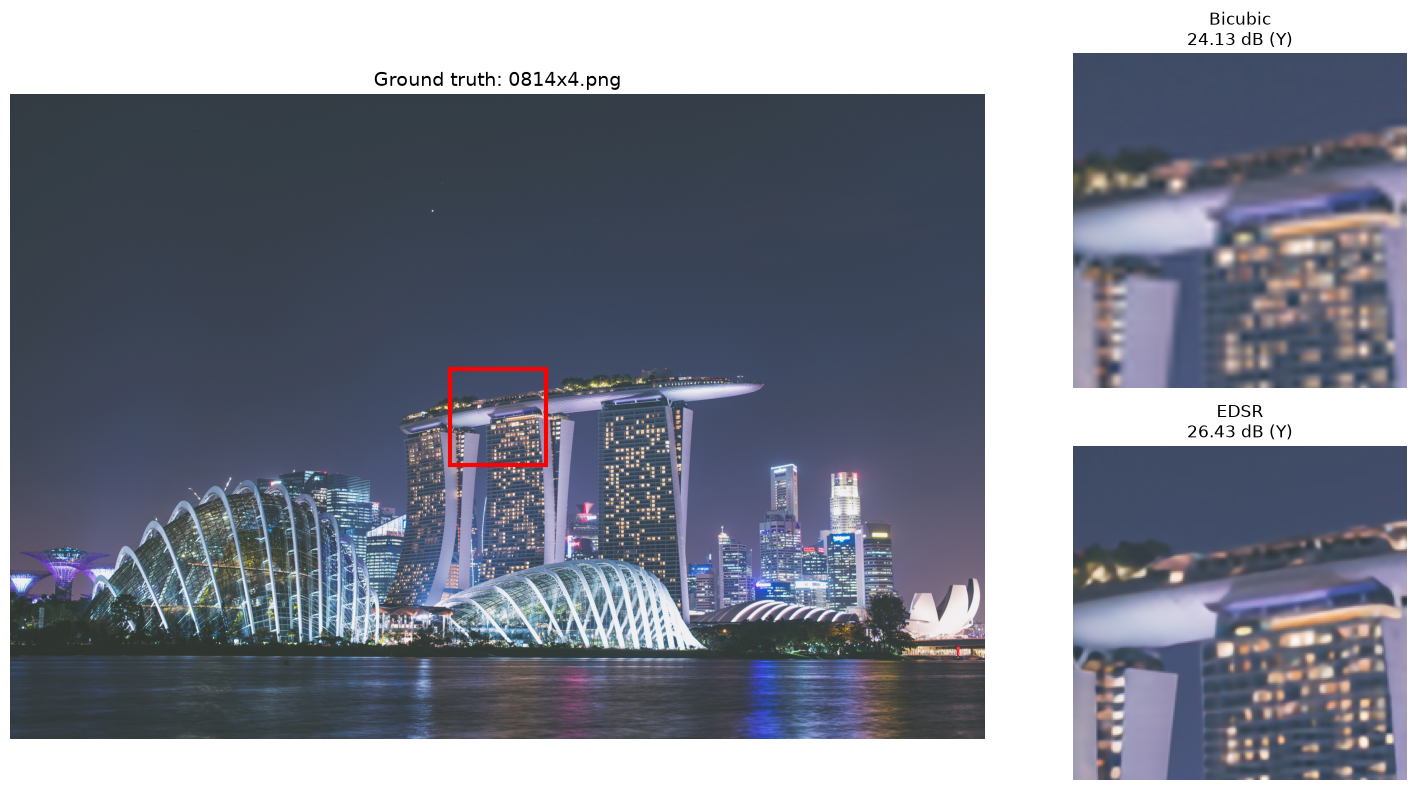
\includegraphics[width=\linewidth]{city.png}\\[0.3ex]
      {\color{inkmuted}\large\bfseries 0814\; \textperiodcentered\; geometric structures\; \textperiodcentered\; {\color{vuborange}+2.30 dB}}
    \end{card}
  \end{column}
  \begin{column}{0.327\linewidth}
    \begin{card}
      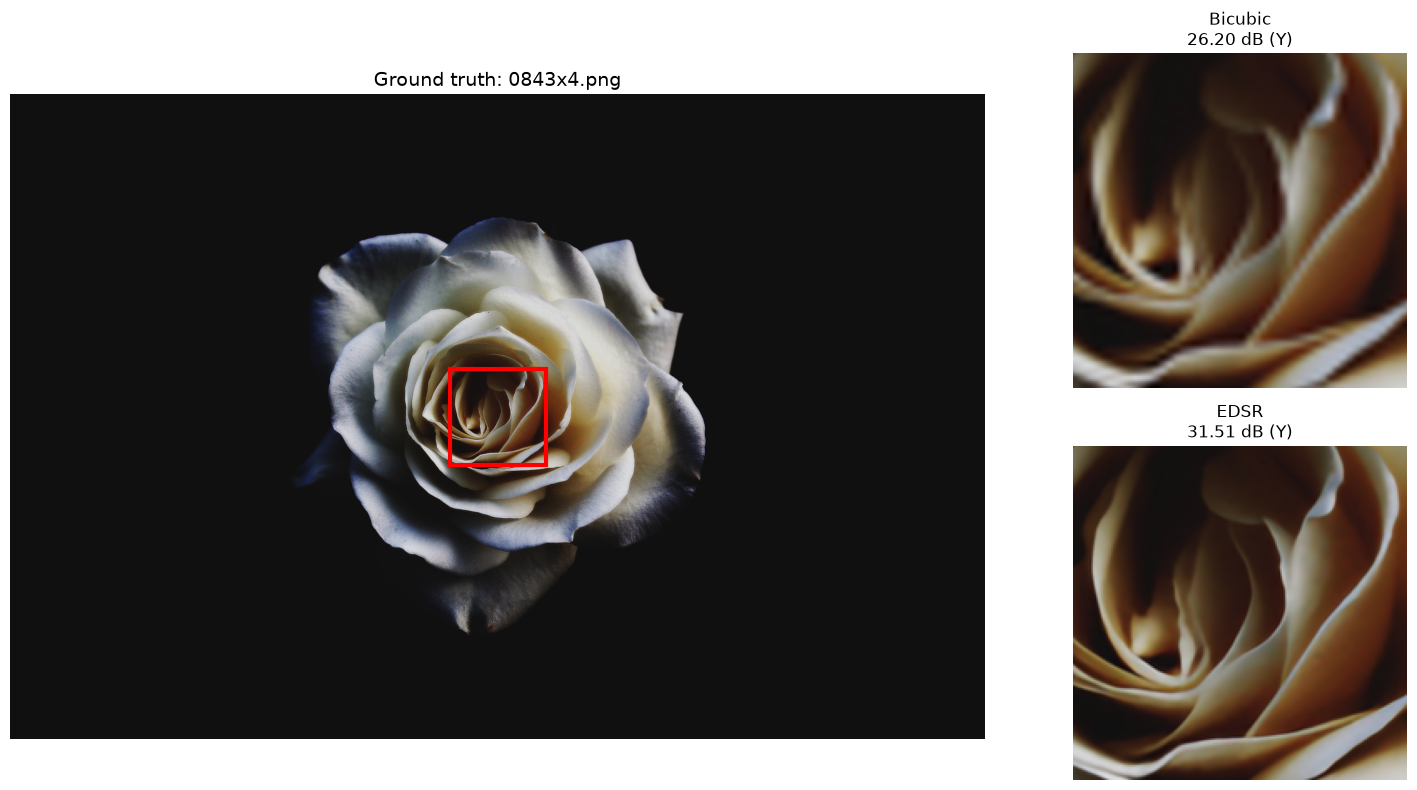
\includegraphics[width=\linewidth]{rose.png}\\[0.3ex]
      {\color{inkmuted}\large\bfseries 0843\; \textperiodcentered\; fine textures\; \textperiodcentered\; {\color{vuborange}+5.31 dB}}
    \end{card}
  \end{column}
  \begin{column}{0.327\linewidth}
    \begin{card}
      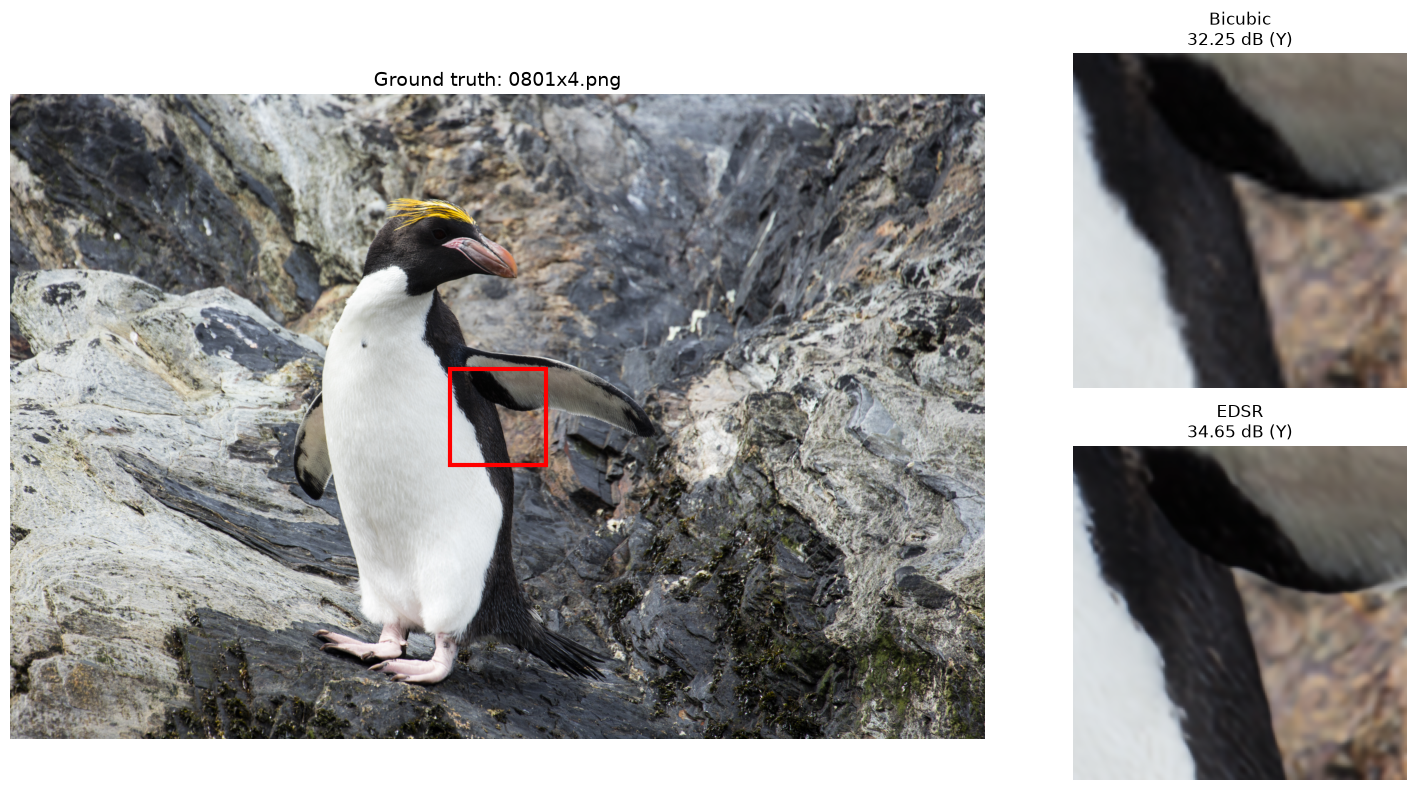
\includegraphics[width=\linewidth]{penguin.png}\\[0.3ex]
      {\color{inkmuted}\large\bfseries 0801\; \textperiodcentered\; edges and fur\; \textperiodcentered\; {\color{vuborange}+2.40 dB}}
    \end{card}
  \end{column}
\end{columns}

\vfill

% ================= FOOTER =================
{\color{inkmuted}\large\bfseries
 Vrije Universiteit Brussel\; \textperiodcentered\; MACS\; \textperiodcentered\; August 2026
 \hfill
 Trained on the VUB ETRO GPU farm\; \textperiodcentered\; 4$\times$ NVIDIA A100}
\vspace{0.8em}

\end{frame}
\end{document}
